\documentclass[10pt,onecolumn,conference]{IEEEtran}
\usepackage{amssymb,amsmath}
\usepackage{graphicx,subfigure}
\graphicspath{ {../img/} }
\hyphenation{op-tical net-works semi-conduc-tor}
\begin{document}
\title{Explore Trust-based Matrix Factorization for Recommendation System}
\author{\IEEEauthorblockN{ZHAO Huan}\\
\IEEEauthorblockA{Department of Computer Science and Engineering, HKUST\\
hzhaoaf@cse.ust.hk\\
ID:20223866}
}

\maketitle

\IEEEpeerreviewmaketitle



\section{Introduction}
% no \IEEEPARstart
Nowadays we are in the era of big data with the development of all kinds of web services. However, it brings about an increasing problem-information overload, which makes it difficult for us to obtain the information we need.For example, according to \cite{stats_url} in just one minute, YouTube users upload 300 hours of new video, Facebook users like 4,166,667 posts, Instagram users like 1,736,111 photos, Snapchat users share 284,722 snaps, and Pinterest sees 9,722 users Pin images. Under this condition, it's very likely for us to get overwhelmed by the flood of information.To address this problem, people both in academia and industry seek for the help of Recommendation System(RS), which is a technique of information filter, aiming at providing users with items(movies, books, music, news, Web pages, etc) based on their interests. Due to its huge commercial value, RS has been successfully in industry,such as product recommendation at Amazon and movie recommendation at Netflix, etc. 

Collaborative Filtering (CF), one popular method for RS, tries to predict users' ratings in unseen items by collecting their rating information from other similar users or items. The underlying assumption of CF is that people will be fond of the items that are similar to those they liked in the past, or that similar users prefer. Generally, CF are roughly categorized into memory-based and model-based methods. Memory-based methods mainly utilize the neighborhood information of users or items in the user-item rating matrix while model-based methods try to use techniques in Machine Learning, Data Mining to discovery the latent factors that affect the rating. Despite the simplicity of memory-based methods, the model-based methods have better predicting performance. And among the various model-based methods, matrix factorization(MF) has become one of the most popular ones in recent years, due to its good performance and scalability in large datasets. \cite{koren2009matrix}\cite{mnih2007probabilistic}.

MF mainly deals with the rating prediction task in RS. For example, at Netflix, a typical user will give a rating(from 1 to 5) to a movie after watching. Then Netflix will predict the rating a user will give to an unseen movie according to his or her rating history. The process is done in the user-item matrix  $R \in \mathbb{R}^{m \times n}$, where $m$ represents the number of users and $n$ represents the number of items. Based on an assumption that a user's rating is governed by a small amount of latent factors, the rating matrix $R$ can be approximated by a multiplication of l-rank factors,
\begin{equation}
R \approx U^TV,
\end{equation}
where $U \in \mathbb{R}^{l \times m}$ and {$U \in \mathbb{R}^{l \times m}$} with $l < min(m, n)$, representing latent feature of items and users' preference, respectively. Traditionally, The Singular Value Decomposition (SVD) method is utilized to approximate a rating matrix $R$ by minimizing
\begin{equation}
\frac{1}{2}||R - U^TV||_F^2,
\end{equation}
where $||\cdot||_F^2$ denotes the Frobenius norm. However, due to the fact that R contains a large number of missing values, we only need to factorize the observed ratings in matrix R. Hence, we change Equation (2) to
\begin{equation}
\min_{U,V}\frac{1}{2}\sum_{i=1}^{m}\sum_{j=1}^{n}I_{ij}(R_{ij} - U_i^TV_j)^2,
\end{equation} 
where $I_{ij}$ is the indicator function that is equal to 1 if user $u_i$ rated item $v_j$ or equal to 0 otherwise. In order to avoid overfiting, two regularization terms are added into Equation (3). Hence we have
\begin{equation}
\min_{U,V}\frac{1}{2}\sum_{i=1}^{m}\sum_{j=1}^{n}I_{ij}(R_{ij} - U_i^TV_j)^2 + \frac{\lambda_1}{2}||U||_F^2 + \frac{\lambda_2}{2}||V||_F^2,
\end{equation} 
where $\lambda_1, \lambda_2 > 0 $.This optimization problem in Equation (4) minimizes the sum-of-squared-errors objective function with quadratic regularization terms, which can be solved by a gradient descent method. After getting $U$ and $V$, then the missing value in the rating matrix $R$ can be predicted in the following:
\begin{equation}
R_{ij} = U_i^TV_j,
\end{equation}
in which, $R_{ij}$ represents the rating to the item $v_j$ given by the user $u_i$, and $U_i$ and $V_i$ represent the corresponding latent factors, respectively.

Despite the good performance of MF, there are two main challenges facing it. The first one is called cold start, which is caused by new items without any ratings or users without any behaviors, thus it is difficult to predict the latent factors. The second one is the sparsity, since most users only rate a small amount of items thus making the rating matrix very sparse.

To address these two problems, one popular approach is to integrate side information into the MF framework. Recently, based on the intuition that users' ratings can be influenced by his friends or people he trusts in social network, a few social-aware or trust-aware recommendation methods have been proposed in \cite{jamali2010matrix}\cite{ma2009llearningEnsembel}\cite{ma2009learningTrust}\cite{ma2008sorec}\cite{ma2011recommender}\cite{massa2004trust}\cite{yang2013social}. More specially, when a user is rating, he may align with his friends or people he trust. Thus, in order to model this, \cite{jamali2010matrix}\cite{ma2009llearningEnsembel}\cite{ma2009learningTrust}\cite{ma2008sorec}\cite{ma2011recommender}\cite{massa2004trust} firstly try to quantify the value of social or trust, and then integrating them into the MF framework by adding regularizations. The new objective function then become
\begin{equation}
\min_{U,V}\frac{1}{2}\sum_{i=1}^{m}\sum_{j=1}^{n}I_{ij}(R_{ij} - U_i^TV_j)^2 + \frac{\beta}{2}\sum_{i=1}^{m}\sum_{f \in \phi(U_i)}\gamma(U_i, U_f)||U_i - U_f||_F^2 + \frac{\lambda_1}{2}||U||_F^2 + \frac{\lambda_2}{2}||V||_F^2,
\end{equation} 
where $\phi(U_i)$ represents the set of users that user $u_i$ trust or have connections, $\gamma(U_i,U_f)$ is a function that measures the intensity of the trust or connections between two users. The regularization term $\frac{\beta}{2}\sum_{i=1}^{m}\sum_{f \in \phi(U_i)}\gamma(U_i, U_f)||U_i - U_f||_F^2$ can be explained by the fact that a user's rating should be close to people he trusts or have connections.

\section{Related Work}
\subsection{Matrix Factorization}
In this section, we review some existing work on recommendation system with matrix factorization techniques, integrating social trust. Firstly, matrix factorization has been one of most popular approaches in the domain of collaborative filtering, which is traditionally one of the typical methods for recommendation system. In collaborative filtering, there are a set of m users $\mathcal{U} = \{u_1,u_2,...,u_m\}$ and a set of n items $\mathcal{I} = \{i_1,i_2,...,i_n\}$, where each user $u_i$ may express their preference to some items by giving a rate in a range. For example, in Netflix, users will rate the movies from 1 to 5 start they watched to show how much they like the movie. Therefore, the rating matrix $R \in \mathbb{R}^{m \times n}$ is formed, in which the rows and columns represent the users and items, respectively. And an entry in R $R_ij$ records the rating user $U_i$ gave to the item $I_j$. 

In reality, most of the entries in the rating matrix R are unknown because one user only rates a small number of items, making the matrix very sparse. We need to predict the missing ratings a user gives to an item based on his or her history ratings. Matrix Factorization technique, one of the most popular approaches, is based on the assumption that there are a few of latent factors deciding the items' properties and users' preferences. Then the rating $R_ij$ user $U_i$ give to the item $I_j$ can be predicted by the inner product of two latent feature vectors, which is shown in equation (5). Further, the model is trained on the observed rating data by minimizing the square error(with the usual Frobenius/L2-norm regularization), which is the equation (3) and (4)(see also \cite{koren2009matrix}).

In \cite{mnih2007probabilistic}, the author gives a probabilistic explaination to the matrix factorization. They adopt a probabilistic linear model with Gaussian observation noise(see fig.1), and define the conditional distribution over the observed ratings as
\begin{equation}
p(R|U,V,\sigma^2) = \prod_{i=1}^{M}\prod_{j=1}^{N}\big[\mathcal{N}(R_{ij}|U_i^TV_j,\sigma^2)\big]^{I_{ij}},
\end{equation} 
where $\mathcal{N}(R_{ij}|U_i^TV_j,\sigma^2)$ is a probability density function of the Gaussian distribution with mean $\mu$ and variance $\sigma^2$, and $I_{ij}$ is the indicator function that is equal to 1 if user i rated item j and equal to 0 otherwise. Zero-mean spherical Gaussian priors are also placed on user and item feature vectors, 
\begin{equation}
p(U|\sigma_U^2) = \prod_{i=1}^{M}\mathcal{N}(U_{i}|0,\sigma_U^2\bold{I}),\quad\quad
p(V|\sigma_V^2) = \prod_{j=1}^{N}\mathcal{N}(V_{j}|0,\sigma_V^2\bold{I}),
\end{equation} 
Then by maximizing the log of posterior distribution over the user and movie features,
\begin{equation}
ln(p(U,V|R, \sigma^2,\sigma_U^2,\sigma_V^2)) = -\frac{1}{2\sigma^2}\sum_{i=1}^{M}\sum_{j=1}^{N}I_{ij}(R_{ij} - U_i^TV_j)^2 - \frac{1}{2\sigma_U^2}\sum_{i=1}^{M}U_i^TU_i - \frac{1}{2\sigma_V^2}\sum_{j=1}^{N}V_j^TV_j + C,
\end{equation} 
( where C is a constant that does not depend on the parameters) is equivalent to minimizing the sum-of-squared-erros objective function with quadratic regularization terms:
\begin{equation}
\min_{U,V}\frac{1}{2}\sum_{i=1}^{M}\sum_{j=1}^{N}I_{ij}(R_{ij} - U_i^TV_j)^2 + \frac{\lambda_1}{2}||U||_F^2 + \frac{\lambda_2}{2}||V||_F^2,
\end{equation} 
\begin{figure}[h]
	\caption{the graphical representation of Probabilistic Matrix Factorization (PMF)}
	\centering
	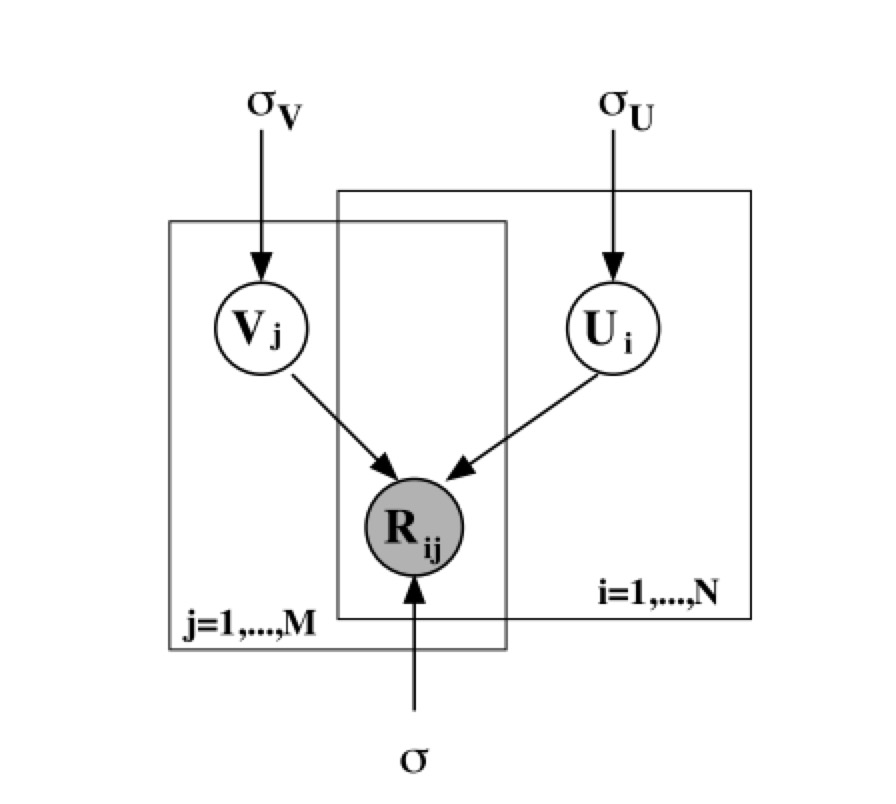
\includegraphics[width=8cm]{pmf}
	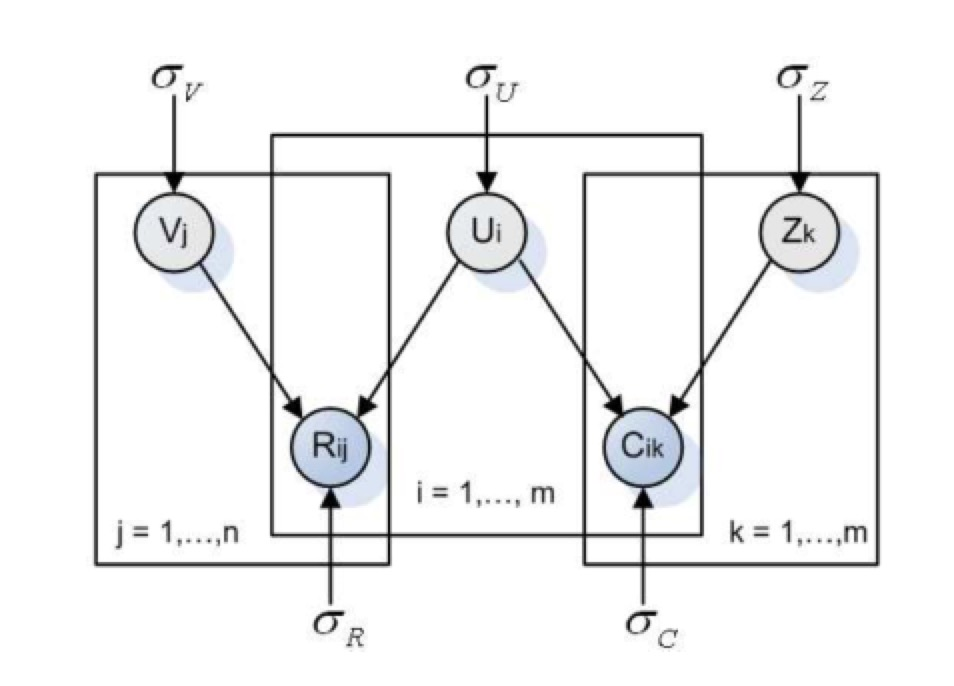
\includegraphics[width=8cm]{sorec}
\end{figure}

\subsection{Matrix Factorization with social networks and trust}
MF and PMF have been the most popular techniques for rating prediction. However, there are two main problems facing them:cold start and sparsity. Cold start problem refer to that new users or items that do not have any ratings. And sparsity refers to the fact that the matrix is sparse. To address these two problems, researchers tried to integrate different side information into the matrix factorization framework, among which the social factors stand out because the booming of online social networks recent years. \cite{jamali2010matrix}\cite{ma2009llearningEnsembel}\cite{ma2009learningTrust}\cite{ma2008sorec}\cite{ma2011recommender}\cite{massa2004trust}\cite{yang2013social}. The underlying assumption of all the work is that users can affect and be affected by his friends when rating an item, while in the standard MF, all the users and items are considered independent and identically distributed(i.i.d).

Apart from the rating matrix R, there is one more matrix $S^{m \times m}$ representing the social network with m nodes, where the nodes represent users and the arcs represent connections between users. $S_{ij}$ is a real value describing the strength of connection between user $U_i$ and $U_j$. In \cite{ma2008sorec}, the SoRec model is proposed to integrate the social network into the probabilistic matrix factorization framework. The two matrices are connected by the assumption that the user latent feature space in the social network matrix is the same in the user\_item rating matrix.(see figure 2).By co-factorizing the rating and social matrix, the low\_rank user\-specific and item\-specific latent features are learned by a similar gradient descent method. There is another underlying assumption that an user's rating are affected by his or her friends in the social networks. The experimental analysis shows the method generates better recommendations than the traditional collaborative filtering algorithms. However, the disadvantage of this work is that it lacks physical interpretations, which does not reflect the real world recommendation process.

Then in \cite{ma2009llearningEnsembel} and \cite{ma2009learningTrust}, Ma et al. further explore how the connections between users affect their rating behaviors. Based on a very intuitive assumption that an user's preferences is closer to the people he or she trusts or likes but farther to those he or she distrusts or dislikes. In \cite{ma2009llearningEnsembel}, the authors interpret one user's final ratings as the balance between this user's own taste and his or her trusted users' favors.Finally, an ensemble probabilistic matrix factorization method is proposed to model this process. The experimental results demonstrate that this approach can better model the problem. In \cite{ma2009learningTrust}, the authors try to incorporate the trust and distrust relations respectively into the rating process. They make the trust and distrust information as regularization terms to the MF objective functions and then perform a similar gradient descent method to calculate the user\-specific and item\-specific latent features. Their experiments shows the improving performance of prediction while an obvious problem facing this method, which is that they just treat distrust the same way as trust. However, in reality, distrust affects people's decision not the same way as trust does. Besides, trust and distrust are regularized respectively thus a very straightforward direction is fuse these two data sources into the same objective function. 

In \cite{jamali2010matrix}, the author extent the work of \cite{ma2009llearningEnsembel} by taking into account trust propagation, which is not considered previously. The model is proposed according to the theory from social influence that the behavior of a user $u$ is affected by his direct neighbors $N_u$. In specific speaking, the latent feature vector of $u$ is dependent on the latent feature vector of all his direct neighbors $v \in N_u$. Then the influence is formulated as 
\begin{equation}
\widehat{U}_u = \frac{\sum_{v \in N_u} T_{u,v}U_u}{\sum_{v \in U_u}T_{u,v}} = \frac{\sum_{v \in N_u} T_{u,v}U_u}{|N_u|},
\end{equation}
where $\widehat{U}_u$ is the estimated latent feature vector of $u$ given the feature vectors of his direct neighbors. Recursively, the latent feature vector of each direct neighbor is dependent on the feature vector of his direct neighbors, leading to the propagation of trust. Finally, a very similar objective function to that in \cite{ma2009learningTrust} is given and it is also calculated by gradient descend method. The performance is also improved in two real datasets, which demonstrates the effectiveness of the exploition of trust propagation. An potential improving direction of this work is to handle distrust relations, whose propagation is surely different from trust.

So far, three general techniques are employed to incorporate the social factors: co-factorization \cite{ma2008sorec} and regularization \cite{ma2009learningTrust}\cite{jamali2010matrix} and ensemble method\cite{ma2009llearningEnsembel}. Actually, the following work of this direction are mostly utilizing these three techniques. In \cite{ma2011recommender}, Ma et al. systematically illustrate how to design a matrix factorization objective function with social regularization, which can also be easily extended to incorporate other side information like contextual information, social tags, etc. Two regularization terms are proposed in this work. One is average-based, whose underlying assumption is that every user's taste is close to the average taste of this user's friends. The other one is individual-based, which requires that the more similar two users are, the closer their latent features should be. The advantage of this work is not only improving the performance of recommendation, but also give a general way to incorporate side information to MF framework. All of the following work \cite{Forsati:2015:PER:2792838.2800198} \cite{li2015overlapping} \cite{yang2013social} use a similar regularization method to incorporate other side information into the MF framework and improves the performance.

In summary, all the aforementioned approaches are regarding the social or trust relations as side information to address the cold start and sparsity. And experiments in real datasets demonstrate the effectiveness of these methods. One underlying assumption all the methods share is that one user will be affected by his/her friends in social network or trust people in all aspects. However, this is no always true. In \cite{yang2012circle}, X. Yang et al. argue that a user may trust different subsets of friends regrading different domains. For example, we may ask some friends for recommendations when buying cars while others when buying cellphones. In other words, the trust is domain- or category- specific. Therefore, the authors propose a circle-based matrix factorization framework, which tries to infer category\-specific social trust circles from the rating data combined with social network data where social trust links across all categories are mixed together. However, the method need to utilize the category information of items while in most cases they are not accessible. Therefore, an category inferring approaches are proposed in this paper, which tries to learn the implicit domain-specific trust.





\section{Preliminary ideas}
Apart from the existing work considering trust or social connections as side information to improve the performance of RS, I will dive deeper into utilizing the trust information based on an intuition that we trust different friends in different domains. For example, we usually seek for advices on movies and cars recommendation from different friends just depending on how much we trust them in the corresponding domain. Therefore, it's not that accurate for the previous work, which directly considers the trust in the whole.

Another idea comes from a fact that previous work rely on explicit trust claimed in the dataset like Epinion\footnote{http://www.public.asu.edu/~jtang20/datasetcode/truststudy.htm} while in most online social networks, the explicit trust are not accessible. This leads to an very straightforward concern on inferring implicit trust according to users' social connections and behaviors history.Therefore, new methods will be proposed to model the implicit trust.

In summary, I will continue working on integrating trust into existing MF framework for RS. However, my focus will be on domain-specific and implicit trust, which will surely be novel to previous work.

\bibliographystyle{abbrv}
\bibliography{ref}
\end{document}


